\pdfbookmark{Общая характеристика работы}{characteristic}             % Закладка pdf
\section*{Общая характеристика работы}

\newcommand{\actuality}{\pdfbookmark[1]{Актуальность}{actuality}\textbf{\actualityTXT}}
\newcommand{\progress}{\pdfbookmark[1]{Степень разработанности темы исследования}{progress}\textbf{\progressTXT}}
\newcommand{\aim}{\pdfbookmark[1]{Цели}{aim}{\textbf\aimTXT}}
\newcommand{\tasks}{\pdfbookmark[1]{Задачи}{tasks}\textbf{\tasksTXT}}
\newcommand{\aimtasks}{\pdfbookmark[1]{Цели и задачи}{aimtasks}\aimtasksTXT}
\newcommand{\novelty}{\pdfbookmark[1]{Научная новизна}{novelty}\textbf{\noveltyTXT}}
\newcommand{\passport}{\pdfbookmark[1]{Соответствие паспорту специальности.}{passport}\textbf{\passportTXT}}
\newcommand{\theorinfluence}{\pdfbookmark[1]{Теоретическая значимость}{theorinfluence}\textbf{\theorinfluenceTXT}}
\newcommand{\influence}{\pdfbookmark[1]{Практическая значимость}{influence}\textbf{\influenceTXT}}
\newcommand{\methods}{\pdfbookmark[1]{Методология и методы исследования}{methods}\textbf{\methodsTXT}}
\newcommand{\defpositions}{\pdfbookmark[1]{Положения, выносимые на защиту}{defpositions}\textbf{\defpositionsTXT}}
\newcommand{\integration}{\pdfbookmark[1]{Внедрение}{integration}\textbf{\integrationTXT}}
\newcommand{\reliability}{\pdfbookmark[1]{Достоверность}{reliability}\textbf{\reliabilityTXT}}
\newcommand{\probation}{\pdfbookmark[1]{Апробация}{probation}\textbf{\probationTXT}}
\newcommand{\contribution}{\pdfbookmark[1]{Личный вклад}{contribution}\textbf{\contributionTXT}}
\newcommand{\publications}{\pdfbookmark[1]{Публикации}{publications}\textbf{\publicationsTXT}}


{\actuality} Задача ранжирования набора данных по некоторым заданным метрикам является одной из приоритетных задач анализа и обработки информации.
Существует множество областей и подходов, направленных на решение этих задач.
Однако, не всегда методы, которые были разработаны для определенных математических моделей, могут быть экстраполированы на другие.
Поэтому, остаются научные области, которые требуют развития принципиально новых подходов для решения задачи ранжирования и выделения релевантной информации.

% Подводка к существующим проблемам:
% 1) В целом рост числа экспериментов
% 2) Усложнение дизайна

Примером такой научной области является системная биология, где ежегодно наблюдается прирост проводимых экспериментов по анализу организации и взаимодействия генов.
Такие эксперименты принято называть экспериментами по анализу \textit{экспрессии генов}.
При этом ситуация не ограничивается простым ростом проводимых экспериментов, а также наблюдается тенденция их усложнения.
Это выражается усложнением структур данных, которые используются для описания этих экспериментов.

Классическим подходом анализа экспериментов экспрессии генов является применение методов математической статистики и вычислительных алгоритмов.

Объектами, к которым применяются методы и алгоритмы являются числовые матрицы, описывающие биологические эксперименты.
При этом исследователей интересует насколько неслучайны свойства того или иного набора генов, где набор генов - это всего лишь некоторое подмножество строк матрицы.
Классические методы в этой области работают в предположении о том, что столбцы матрицы соответствуют двум группам биологических образцов.
Это приводит к невозможности прямолинейного применения существующих методов для числовых матриц, в которых имеется более двух различных групп образцов.
Соответствие столбцов матриц биологическим образцам носит название \textit{аннотации эксперимента}.


В настоящее время, исследователи зачастую предоставляют открытый доступ к результатам своих экспериментов.
Для систематизации таких данных были разработаны специальные публично открытые базы данных.
Открытые базы данных с большим числом экспериментальных данных открывают широкие возможности для повторного использования и анализа результатов экспериментов, что позволяет решить сразу несколько задач.
Во-первых, это открывает исследователям возможность находить схожие эксперименты в терминах экспрессии генов, которые в своей основе имеют различные биологические предпосылки.
Как результат, такие ситуации позволяют формулировать новые биологические гипотезы, затем валидировать их путем проведения дополнительных экспериментов и тем самым раскрывать новые биологические закономерности.
Во-вторых, использование вычислительных методов, направленных на повторный анализ существующей информации, оказывается экономически выгоднее, нежели прямолинейное проведение биологического эксперимента.



Таким образом, разработка и исследование системы поиска релевантных биологических экспериментов является актуальной задачей в области системной биологии и области анализа информации. 
Разработка и применение поисковых систем потенциально позволит формулировать и обнаруживать новые биологические механизмы, лежащие в основе процессов, протекающих в живых организмах.

% \ifsynopsis
% Этот абзац появляется только в~автореферате.
% Для формирования блоков, которые будут обрабатываться только в~автореферате,
% заведена проверка условия \verb!\!\verb!ifsynopsis!.
% Значение условия задаётся в~основном файле документа (\verb!synopsis.tex! для
% автореферата).
% \else
% Этот абзац появляется только в~диссертации.
% Через проверку условия \verb!\!\verb!ifsynopsis!, задаваемого в~основном файле
% документа (\verb!dissertation.tex! для диссертации), можно сделать новую
% команду, обеспечивающую появление цитаты в~диссертации, но~не~в~автореферате.
% \fi

% {\progress}
% Этот раздел должен быть отдельным структурным элементом по
% ГОСТ, но он, как правило, включается в описание актуальности
% темы. Нужен он отдельным структурынм элемементом или нет ---
% смотрите другие диссертации вашего совета, скорее всего не нужен.


{\progress} Существует ряд методов, которые решают задачу анализа экспрессии генов в рамках одного биологического эксперимента.
Одним из популярных и широко используемых методов является Gene Set Enrichment Analysis (GSEA).
В выпускной квалификационной работе \cite{KorotkevichVKR} был рассмотрен прототип метода вычисления произвольно малых P-значений с хорошей относительной точностью, что являлось основным недостатком оригинального метода GSEA.
Этот метод позволяет быстро вычислять сколь угодно малые P-значения и основан на применении многоуровневого метода Монте-Карло.
Однако в работе не было досконально изучена накапливаемая ошибка и степень сходимости метода для различных практических приложений.

{\aim} данной работы является создание эффективной системы поиска биологических экспериментов в открытых базах данных на основе обнаружения наборов генов с высокой попарной корреляцией значений экспрессии.

Для~достижения поставленной цели необходимо было решить следующие {\tasks}:
\begin{enumerate}[beginpenalty=10000] % https://tex.stackexchange.com/a/476052/104425
  \item Разработка подхода эффективного оценивания вероятностей редких событий при проверке статистических гипотез для наборов генов.
  \item Определение статистики для экспериментов с произвольным числом групп образцов и использование подхода, полученного в рамках задачи 1, для проверки статистических гипотез для введенной статистики.
  \item Разработка системы поиска биологических экспериментов по заданному набору генов среди открытых баз данных экспериментов по анализу экспрессии генов на основе статистики, предложенной в рамках задачи 2.
\end{enumerate}


{\novelty}
\begin{enumerate}[beginpenalty=10000] % https://tex.stackexchange.com/a/476052/104425
    \item Был предложен подход эффективного оценивания вероятностей редких событий для наборов генов.
    В отличие от существующих, данный подход позволяет использовать различные типы статистик для исследуемых наборов генов и вычислять произвольно малые P-значения. 
    Подход имеет критерий остановки для процесса оценивания P-значений, а также имеет оценку точности результатов работы.
    \item Определена статистика для набора генов, которая не зависит от наличия аннотации биологического эксперимента.
    Введенная статистика позволила разработать метод, который в отличие от известных, позволяет в автоматическом режиме проверять статистические гипотезы при анализе биологических экспериментов и не требует наличия аннотации для экспериментов.
    \item Реализована оригинальная поисковая система для поиска релевантных биологических экспериментов для заданного набора генов.
    В отличие от существующих систем, где результатом являются курированные наборы генов, реализованная система возвращает ранжированный список экспериментов. Данная система позволяет эффективно осуществлять поиск среди больших баз данных публично доступных результатов биологических экспериментов.
\end{enumerate}

{\defpositions}
\begin{enumerate}[beginpenalty=10000] % https://tex.stackexchange.com/a/476052/104425
    \item Для решения задачи 1 был разработан подход оценки вероятностей редких событий для наборов генов при отклонении тестовой статистики от нулевой гипотезы.
    \item Для решения задачи 2 был разработан новый метод Gene Set Co-Regulation Analysis (GESECA). Метод позволяет в автоматическом режиме осуществлять анализ статистической значимости в независимости от наличия аннотаций биологического эксперимента.
    \item На основе разработанного метода GESECA была разработана система поиска биологических экспериментов. Поисковая система принимает на вход произвольный набор генов и возвращает ранжированный список биологических экспериментов. Эксперименты ранжируются по P-значениям, полученным после применения метода GESECA. 
\end{enumerate}


{\passport} Работа соответствует паспорту специальности 05.13.17 - <<Теоретические основы информатики>> и относится к пункту 9: <<Разработка новых интернет-технологий, включая средства поиска, анализа и фильтрации информации, средства приобретения знаний и создания онтологии, средства интеллектуализации бизнес-процессов.>>.

{\theorinfluence} состоит в формулировке подхода оценивания произвольно малых P-значений при проверке статистических гипотез для наборов генов. Предложен критерий остановки для процесса оценивания P-значений и осуществлен корректный переход к вычислению логарифмов P-значений.

{\influence} состоит в том, что реализованный метод GESECA и поисковая система могут быть использованы для упрощения процесса анализа и исследования биологических процессов, протекающих в живых организмах. 
Также они позволяют исследователям синтезировать абсолютно новые предположения о биологических закономерностях, и находить подтверждения для гипотез, сформированных раннее. 

{\methods} В работе используются методы обработки информации, преобразования информации в данные и знания.

% В папке Documents можно ознакомиться с решением совета из Томского~ГУ
% (в~файле \verb+Def_positions.pdf+), где обоснованно даются рекомендации
% по~формулировкам защищаемых положений.

{\reliability} полученных результатов обеспечивается корректно поставленными задачами, а также большим числом проведенных численных экспериментов.
Полученные результаты находятся в хорошем соответствии с результатами других ислледователей, которые были получены при определенных ограничениях на свойствах исследуемых ими объектах.

{\integration} Разработанный подход эффективного оценивания вероятностей редких событий при проверке статистических гипотез для наборов генов позволил реализовать метод Fast Gene Set Enrichment Analysis Multilevel (FGSEA-Multilevel).
Метод был внедрен в пакет fgsea, написанный на языках программирования R и C++. 
Данный пакет является свободно доступным и размещен в архиве биологических пакетов Bioconductor (\url{https://www.bioconductor.org/}).
При этом пакет fgsea входит в число наиболее популярных пакетов из всех доступных пакетов в архиве.
Так в настоящее время ранг пакета по числу обращений и скачиваний равен 38-ми из более чем 2000 различных пакетов, представленных в Bioconductor.
Разработанный метод GESECA также является свободно доступным и может быть скачан с github-репозитория по адресу \url{https://github.com/ctlab/fgsea/tree/geseca}. Поисковая система релевантных биологических экспериментов по заданному набору генов реализована в виде веб-сервиса и доступна по адресу \url{https://ctlab.itmo.ru/geseca/}. Все разработанные методы активно применяются в процессе подготовки магистров по программе <<Биоинформатика и системная биология>> в Университете ИТМО.


{\probation}
Основные результаты работы докладывались на:
\begin{enumerate}
    \item Всероссийский конгресс молодых ученых Университета ИТМО, 2019 г., Университет ИТМО, Санкт-Петербург.
    \item Всероссийская научная конференция по проблемам информатики СПИСОК-2019. 2019 г., СПбГУ, Санкт-Петербург.
    \item Moscow Conference on Computational Molecular Biology (MCCMB 2019), 2019 г., Москва.
    \item Всероссийский конгресс молодых ученых Университета ИТМО, 2020 г., Университет ИТМО, Санкт-Петербург
    \item CSHL Meeting on Biological Data Science 2020,  2020 г., онлайн конференция.
    \item Moscow Conference on Computational Molecular Biology (MCCMB 2021). 2021 г., Москва.
    \item Научная и учебно-методическая конференция Университета ИТМО, 2022 г., Университет ИТМО, Санкт-Петербург.
\end{enumerate}

{\contribution} Автор принимал активное участие в процессе анализа и совершенствования метода FGSEA-Multilevel. 
Автором были определены требуемые параметры для сходимости метода при приложениях его для практических задач. 
Был осуществлен анализ теоретических свойств распределения P-значений и совершен корректный переход к вычислениям логарифмов P-значений в методе FGSEA-Multilevel.
Автор принимал активное участие во всех этапах, связанных с разработкой и реализацией метода GESECA, совместно с Сергушичевым~А.А. и Артемовым~М.Н.
Диссертантом была полностью написана программная реализация метода GESECA.
Проведены валидация и верификация корректности работы метода на практике.
Автором разработан веб-сервис, который служит поисковой системой для поиска релевантных экспериментов по заданному набору генов.

\ifnumequal{\value{bibliosel}}{0}
{%%% Встроенная реализация с загрузкой файла через движок bibtex8. (При желании, внутри можно использовать обычные ссылки, наподобие `\cite{vakbib1,vakbib2}`).
    {\publications} Основные результаты по теме диссертации изложены
    в~XX~печатных изданиях,
    X из которых изданы в журналах, рекомендованных ВАК,
    X "--- в тезисах докладов.
}%
{%%% Реализация пакетом biblatex через движок biber
    \begin{refsection}[bl-author, bl-registered]
        % Это refsection=1.
        % Процитированные здесь работы:
        %  * подсчитываются, для автоматического составления фразы "Основные результаты ..."
        %  * попадают в авторскую библиографию, при usefootcite==0 и стиле `\insertbiblioauthor` или `\insertbiblioauthorgrouped`
        %  * нумеруются там в зависимости от порядка команд `\printbibliography` в этом разделе.
        %  * при использовании `\insertbiblioauthorgrouped`, порядок команд `\printbibliography` в нём должен быть тем же (см. biblio/biblatex.tex)
        %
        % Невидимый библиографический список для подсчёта количества публикаций:
        \printbibliography[heading=nobibheading, section=1, env=countauthorvak,          keyword=biblioauthorvak]%
        \printbibliography[heading=nobibheading, section=1, env=countauthorwos,          keyword=biblioauthorwos]%
        \printbibliography[heading=nobibheading, section=1, env=countauthorscopus,       keyword=biblioauthorscopus]%
        \printbibliography[heading=nobibheading, section=1, env=countauthorconf,         keyword=biblioauthorconf]%
        \printbibliography[heading=nobibheading, section=1, env=countauthorother,        keyword=biblioauthorother]%
        \printbibliography[heading=nobibheading, section=1, env=countregistered,         keyword=biblioregistered]%
        \printbibliography[heading=nobibheading, section=1, env=countauthorpatent,       keyword=biblioauthorpatent]%
        \printbibliography[heading=nobibheading, section=1, env=countauthorprogram,      keyword=biblioauthorprogram]%
        \printbibliography[heading=nobibheading, section=1, env=countauthor,             keyword=biblioauthor]%
        \printbibliography[heading=nobibheading, section=1, env=countauthorvakscopuswos, filter=vakscopuswos]%
        \printbibliography[heading=nobibheading, section=1, env=countauthorscopuswos,    filter=scopuswos]%
        %
        \nocite{*}%
        %
        {\publications} Основные результаты по теме диссертации изложены в~\arabic{citeauthor}~печатных изданиях,
        \arabic{citeauthorvak} из которых изданы в журналах, рекомендованных ВАК\sloppy%
        \ifnum \value{citeauthorscopuswos}>0%
            , \arabic{citeauthorscopuswos} "--- в~периодических научных журналах, индексируемых Web of~Science и Scopus\sloppy%
        \fi%
        \ifnum \value{citeauthorconf}>0%
            , \arabic{citeauthorconf} "--- в~тезисах докладов.
        \else%
            .
        \fi%
        \ifnum \value{citeregistered}=1%
            \ifnum \value{citeauthorpatent}=1%
                Зарегистрирован \arabic{citeauthorpatent} патент.
            \fi%
            \ifnum \value{citeauthorprogram}=1%
                Зарегистрирована \arabic{citeauthorprogram} программа для ЭВМ.
            \fi%
        \fi%
        \ifnum \value{citeregistered}>1%
            Зарегистрированы\ %
            \ifnum \value{citeauthorpatent}>0%
            \formbytotal{citeauthorpatent}{патент}{}{а}{}\sloppy%
            \ifnum \value{citeauthorprogram}=0 . \else \ и~\fi%
            \fi%
            \ifnum \value{citeauthorprogram}>0%
            \formbytotal{citeauthorprogram}{программ}{а}{ы}{} для ЭВМ.
            \fi%
        \fi%
        % К публикациям, в которых излагаются основные научные результаты диссертации на соискание учёной
        % степени, в рецензируемых изданиях приравниваются патенты на изобретения, патенты (свидетельства) на
        % полезную модель, патенты на промышленный образец, патенты на селекционные достижения, свидетельства
        % на программу для электронных вычислительных машин, базу данных, топологию интегральных микросхем,
        % зарегистрированные в установленном порядке.(в ред. Постановления Правительства РФ от 21.04.2016 N 335)
    \end{refsection}%
    \begin{refsection}[bl-author, bl-registered]
        % Это refsection=2.
        % Процитированные здесь работы:
        %  * попадают в авторскую библиографию, при usefootcite==0 и стиле `\insertbiblioauthorimportant`.
        %  * ни на что не влияют в противном случае
    \end{refsection}%
        %
        % Всё, что вне этих двух refsection, это refsection=0,
        %  * для диссертации - это нормальные ссылки, попадающие в обычную библиографию
        %  * для автореферата:
        %     * при usefootcite==0, ссылка корректно сработает только для источника из `external.bib`. Для своих работ --- напечатает "[0]" (и даже Warning не вылезет).
        %     * при usefootcite==1, ссылка сработает нормально. В авторской библиографии будут только процитированные в refsection=0 работы.
}

% При использовании пакета \verb!biblatex! будут подсчитаны все работы, добавленные
% в файл \verb!biblio/author.bib!. Для правильного подсчёта работ в~различных
% системах цитирования требуется использовать поля:
% \begin{itemize}
%         \item \texttt{authorvak} если публикация индексирована ВАК,
%         \item \texttt{authorscopus} если публикация индексирована Scopus,
%         \item \texttt{authorwos} если публикация индексирована Web of Science,
%         \item \texttt{authorconf} для докладов конференций,
%         \item \texttt{authorpatent} для патентов,
%         \item \texttt{authorprogram} для зарегистрированных программ для ЭВМ,
%         \item \texttt{authorother} для других публикаций.
% \end{itemize}
% Для подсчёта используются счётчики:
% \begin{itemize}
%         \item \texttt{citeauthorvak} для работ, индексируемых ВАК,
%         \item \texttt{citeauthorscopus} для работ, индексируемых Scopus,
%         \item \texttt{citeauthorwos} для работ, индексируемых Web of Science,
%         \item \texttt{citeauthorvakscopuswos} для работ, индексируемых одной из трёх баз,
%         \item \texttt{citeauthorscopuswos} для работ, индексируемых Scopus или Web of~Science,
%         \item \texttt{citeauthorconf} для докладов на конференциях,
%         \item \texttt{citeauthorother} для остальных работ,
%         \item \texttt{citeauthorpatent} для патентов,
%         \item \texttt{citeauthorprogram} для зарегистрированных программ для ЭВМ,
%         \item \texttt{citeauthor} для суммарного количества работ.
% \end{itemize}
% % Счётчик \texttt{citeexternal} используется для подсчёта процитированных публикаций;
% % \texttt{citeregistered} "--- для подсчёта суммарного количества патентов и программ для ЭВМ.

% Для добавления в список публикаций автора работ, которые не были процитированы в
% автореферате, требуется их~перечислить с использованием команды \verb!\nocite! в
% \verb!Synopsis/content.tex!.
 % Характеристика работы по структуре во введении и в автореферате не отличается (ГОСТ Р 7.0.11, пункты 5.3.1 и 9.2.1), потому её загружаем из одного и того же внешнего файла, предварительно задав форму выделения некоторым параметрам

%Диссертационная работа была выполнена при поддержке грантов \dots

%\underline{\textbf{Объем и структура работы.}} Диссертация состоит из~введения,
%четырех глав, заключения и~приложения. Полный объем диссертации
%\textbf{ХХХ}~страниц текста с~\textbf{ХХ}~рисунками и~5~таблицами. Список
%литературы содержит \textbf{ХХX}~наименование.

\pdfbookmark{Содержание работы}{description}                          % Закладка pdf
\section*{Содержание работы}
Во \textbf{введении} приводится аргументация и обоснование актуальности проведенного исследования, произведен анализ и обзор научных источников по исследуемой проблеме, формулируется цель, производится формальная постановка задач, определены научная новизна и практическая значимость представляемой работы.

% обосновывается актуальность исследований, проводимых в рамках данной диссертационной работы, приводится обзор научной литературы по изучаемой проблеме, формулируется цель, ставятся задачи работы, сформулированы научная новизна и практическая значимость представляемой работы.

\textbf{Первая глава} посвящена обзору предметной области, рассмотрению математических моделей, которые используются при описании экспериментов по анализу экспрессии генов.
В главе приводятся основные понятия и определения, которые используются в задачах оценивания вероятностей для наборов генов при проверке статистических гипотез для наборов генов.
В завершении главы приводятся сформулированная цель исследования и производится формальная постановка задач, рассматриваемых в диссертационной работе.

Классическим подходом по анализу наблюдаемой информации в биологии является применение методов математической статистики.
Так, для исследования того или иного процесса обычно прибегают к рассмотрению выборок, которые при правильном построении позволяют делать выводы о свойствах генеральной совокупности. 
В такой постановке, исследователей часто интересует вероятность наблюдения того или иного события в рамках выполнения нулевой гипотезы.

В общем виде задача может быть сформулирована следующим образом: пусть имеется некоторое конечное множество $U = \left(x_1, x_2, \ldots, x_M \right)$ и некоторое подмножество размера $k \in \mathbb{N}$. Также пусть задана некоторая статистика 
\begin{equation*} 
    S(X) \rightarrow \mathbb{R}, \quad X = \{x_{i_1}, x_{i_2}, \ldots x_{i_k} \mid x_{i_j} \in U\}.
\end{equation*}
Тогда задача по определению статистической значимости в рамках выполнения некоторой нулевой гипотезы относительно распределения объектов $S(X)$ заключается в вычислении следующей вероятности:
\begin{equation}\label{pval_generic}
    \mathbb{P} \left(S(X) \geqslant \gamma \right),
\end{equation}
где $X \subset U$ - случайное подмножество размера $k$ и $\gamma \in S(\Omega)$.
Для ряда задач требуется лишь определить является ли вероятность \ref{pval_generic} меньше уровня значимости $\theta \in [0, 1]$.
Обычно в качестве уровня значимости принимают $\theta = 0.05$ или $\theta = 0.01$.
В такой постановке задача может быть решена при помощи использования метода Монте-Карло.
Для этого необходимо сгенерировать выборку $\left(X_1, X_2, \ldots, X_N \right)$ достаточного размера и вместо исходной вероятности рассмотреть оценку вида
\begin{equation}\label{phat_crude}
    \hat{p} = \frac{1}{N} \sum\limits_{j = 1}^{N} \mathrm{I} \{S(X_j) \geqslant \gamma \},
\end{equation}
где $\mathrm{I} \{S(X_j) \geqslant \gamma \}$ - характеристическая функция. 
После этого совершается переход к неравенству $\hat{p} \leqslant \theta$ и принимается решение о принятии или отвержении нулевой гипотезы.
Однако, существуют примеры задач, в которых требуется не только проверить выполнение неравенства, но также определить оценку для значения вероятности.
В случае, когда искомая вероятность экстремально мала, вышеописанный подход не применим.

Одним из примеров таких задач, является определение статистической значимости набора генов по заданному числовому вектору статистик, которые соответствуют степени регуляции конкретного гена.
Классическим методом, решающим эту задачу, является Gene Set Enrichment Analysis (GSEA) \cite{subramanian2005gene}.
Однако, этот метод имеет несколько ограничений.
Во-первых, это скорость работы, которая существенно усложняет процесс проведения быстрого анализа статистической значимости для наборов генов.
Во-вторых, так как метод основан на применении простого метода Монте-Карло это приводит к невозможности вычисления экстремально малых P-значений.
Последний факт играет важную роль, так как это ограничение способно оказывать влияние на выводы относительно статистической значимости исследуемых наборов генов.

В выпускной квалификационной работе \cite{KorotkevichVKR} был предложен приближенный алгоритм, основанный на применении многоуровневого подхода Монте-Карло.
Этот подход позволяет вычислять произвольно малые P-значения за разумное время работы.
Тем не менее, алгоритм был представлен в виде прототипа без детального анализа сходимости его решений при приложениях на практике.
Данный факт требовал дополнительного изучения вопросов его сходимости и верификации получаемых результатов.

В настоящей работе будет исследован вопрос сходимости, получаемых P-значений к истинным и определены параметры метода, которые позволяют утверждать о сходимости метода при приложениях его на практике.
Также, будет показан корректный переход к логарифмам P-значений, который учитывает теоретические свойства распределений случайных величин и будет получено аналитическое выражение для накапливаемой ошибки алгоритма.

Все вышесказанное относится к анализу статистической значимости наборов генов для случая, когда в биологическом эксперименте участвуют строго две группы образцов и имеется числовой вектор статистик.
Однако, удешевление стоимости проведения экспериментов по анализу экспрессии генов привело к появлению экспериментов со сложным дизайном.
Под сложным дизайном подразумевается эксперимент, в котором присутствует большое число (> 2) различных групп образцов.
Это делает невозможным прямое применение вышеописанных методов на практике и требует развития концептуально новых методов для их анализа.


% картинку можно добавить так:
% \begin{figure}[ht]
%     \centerfloat{
%         \hfill
%         \subcaptionbox{\LaTeX}{%
%             \includegraphics[scale=0.27]{latex}}
%         \hfill
%         \subcaptionbox{Knuth}{%
%             \includegraphics[width=0.25\linewidth]{knuth1}}
%         \hfill
%     }
%     \caption{Подпись к картинке.}\label{fig:latex}
% \end{figure}

% Формулы в строку без номера добавляются так:
% \[
%     \lambda_{T_s} = K_x\frac{d{x}}{d{T_s}}, \qquad
%     \lambda_{q_s} = K_x\frac{d{x}}{d{q_s}},
% \]

\textbf{Вторая глава} посвящена разработке подхода эффективного оценивания вероятностей редких событий при проверке статистических гипотез для наборов генов.

Для решения задачи оценивания вероятности (\ref{pval_generic}) для редких событий, предлагается следующий подход, который основан на применении многоуровневого метода Монте-Карло по схеме марковской цепи.
Суть подхода заключается во введении расщепления 
\begin{equation*}
    \min_{X} S(X) = l_0 < l_1 < \ldots < l_t = \gamma.
\end{equation*}
После этого, искомая вероятность может быть переписана следующим образом
\begin{equation*}
    \mathbb{P} \left(S(X) \geqslant \gamma \right) = \prod\limits_{j=1}^{t} \mathbb{P} \left(S(X) \geqslant l_i \mid S(X) \geqslant l_{i - 1} \right).
\end{equation*}
Затем вместо использования одной оценки для вероятности (\ref{pval_generic}) можно рассмотреть оценку для каждого уровня, а именно
\begin{equation*}
    \prod\limits_{j=1}^{t} \mathbb{P} \left(S(X) \geqslant l_i \mid S(X) \geqslant l_{i - 1} \right) \approx \prod_{j = 1}^{t} \hat{p}_j,
\end{equation*}
где $\hat{p}_j$ классическая оценка вероятности метода Монте-Карло. 
В качестве $l_j, j \in \{1, 2, \ldots, t-1\}$ предлагается брать медианы выборок, полученных на каждом уровне.
Для генерирования равномерной выборки для каждого уровня применяется алгоритм Метрополиса.

Краткое описание алгоритма Метрополиса для генерирования равномерной выборки из распределения $\mathrm{P}\left(\cdot \mid S(X) \geqslant l_j \right)$ выглядит следующим образом:
\begin{enumerate}
    \item Устанавливаем счётчик шагов равным нулю.
    \item Начинаем с выборки $X_1, X_2, \ldots X_N$ такой, что $S(X_i) \geqslant l_j$
    \item Последовательно рассматриваем наборы генов из выборки. Для $X_i$ случайным образом выбираем ген $x_k \in X_i$ из набора и заменяем его случайным геном $\hat{x}_k \in U \setminus X_i$. В случае, если замена сохранила условие $S(X_i) \geqslant l_j, \ i \in \{1, 2, \ldots, N \}$, тогда увеличиваем счетчик шагов на единицу, в противном случае отменяем изменения без инкрементирования счетчика шагов.
\end{enumerate}
От числа шагов напрямую зависит корректность вычисляемой оценки для вероятности $\mathrm{P}\left(\cdot \mid S(X) \geqslant l_j \right)$.
Для случая, когда известны истинные значения вероятностей становится возможным определения необходимого числа шагов для утверждения сходимости оценок к истинным значениям.
В качестве критерия сходимости метода в таких случаях предлагается использовать следующий подход. Оценка P-значения должна попасть в интервал $\left(\mathrm{P}_{\text{true}} - 2 \cdot \mathrm{SEM}, \mathrm{P}_{\text{true}} + 2 \cdot \mathrm{SEM}\right)$, где $\mathrm{P}_{\text{true}}$ - истинное значение вероятности, а $\mathrm{SEM}$ - стандартная ошибка среднего.

На практике при вычислении вероятностей бывает удобно перейти к вычислению логарифма вероятности.
Однако, прямое применение функции логарифма к выражению $\mathrm{P} \left(S(X) \geqslant \gamma \right) \approx \hat{p}_1 \cdot \hat{p}_2 \cdot \ldots \cdot \hat{p}_t $ приводит к тому, что оценка перестает быть несмещенной.
Для корректного перехода необходимо учесть свойство распределения медианы $m$ выборки размера $N$ из равномерного распределения, которое утверждает что в таком случае $m$ соответствует бета-распределению с параметрами $\mathrm{B} \left((N + 1) / 2, (N + 1)/ 2 \right)$. Тогда, несмещенная оценка для логарифма P-значения:
\[
    \log \mathrm{P} \left(S(X) \geqslant \gamma \right) \approx (t - 1) \cdot \left( \psi \left( \frac{N + 1}{2}\right) - \psi \left(N + 1 \right)\right) + \log (\hat{p}_t),
\]
где $\psi$ - дигамма-функция.

Схожим образом мы можем вычислить дисперсию для оценки $\mathrm{D} \left[\log \hat{p}_i \right]= \psi_1 \left(\frac{N + 1}{2}\right) - \psi_1 \left( N + 1 \right)$, где $\psi_1$ тригамма-функция. Отсюда получаем стандартное отклонение нашей оценки:
\[
    \mathrm{sd} = \sqrt{t \cdot \left( \psi_1 \left(\frac{W+1}{2}\right) - \psi_1 \left(W + 1\right)\right)}.    
\]

Вышеописанный подход является обобщением подхода описанного в работе \cite{KorotkevichVKR} для случая общего вида статистики.
При этом предложен критерий для анализа сходимости подхода для ряда задач, в которых известны истинные P-значения.
Также за счёт использования стандартного отклонения оценки можно делать выводы о точности получаемых результатов на практике.

Применение этого подхода для задачи анализа представленности функциональных наборов генов \cite{KorotkevichVKR}, позволило реализовать метод FGSEA-Multilevel.
Входными данными метода являются: массив статистик для генов и коллеция наборов генов.
Для определения необходимого числа шагов алгоритма Метрополиса в методе FGSEA-Multilevel рассматривалась величина вида $\text{steps} = a \cdot k \cdot N$, здесь $N$ - размер выборки, $k$ - размер тестируемого набора генов, $a$ - параметр, который варьировался.
Было продемонстрировано, что для практических применений алгоритма достаточно положить $a = 1$.
Результаты работы алгоритма в зависимости от числа шагов steps продемонстрированы для наборов генов различных размеров на рисунке \ref{fig:pval_error}.

\begin{figure}[h]
    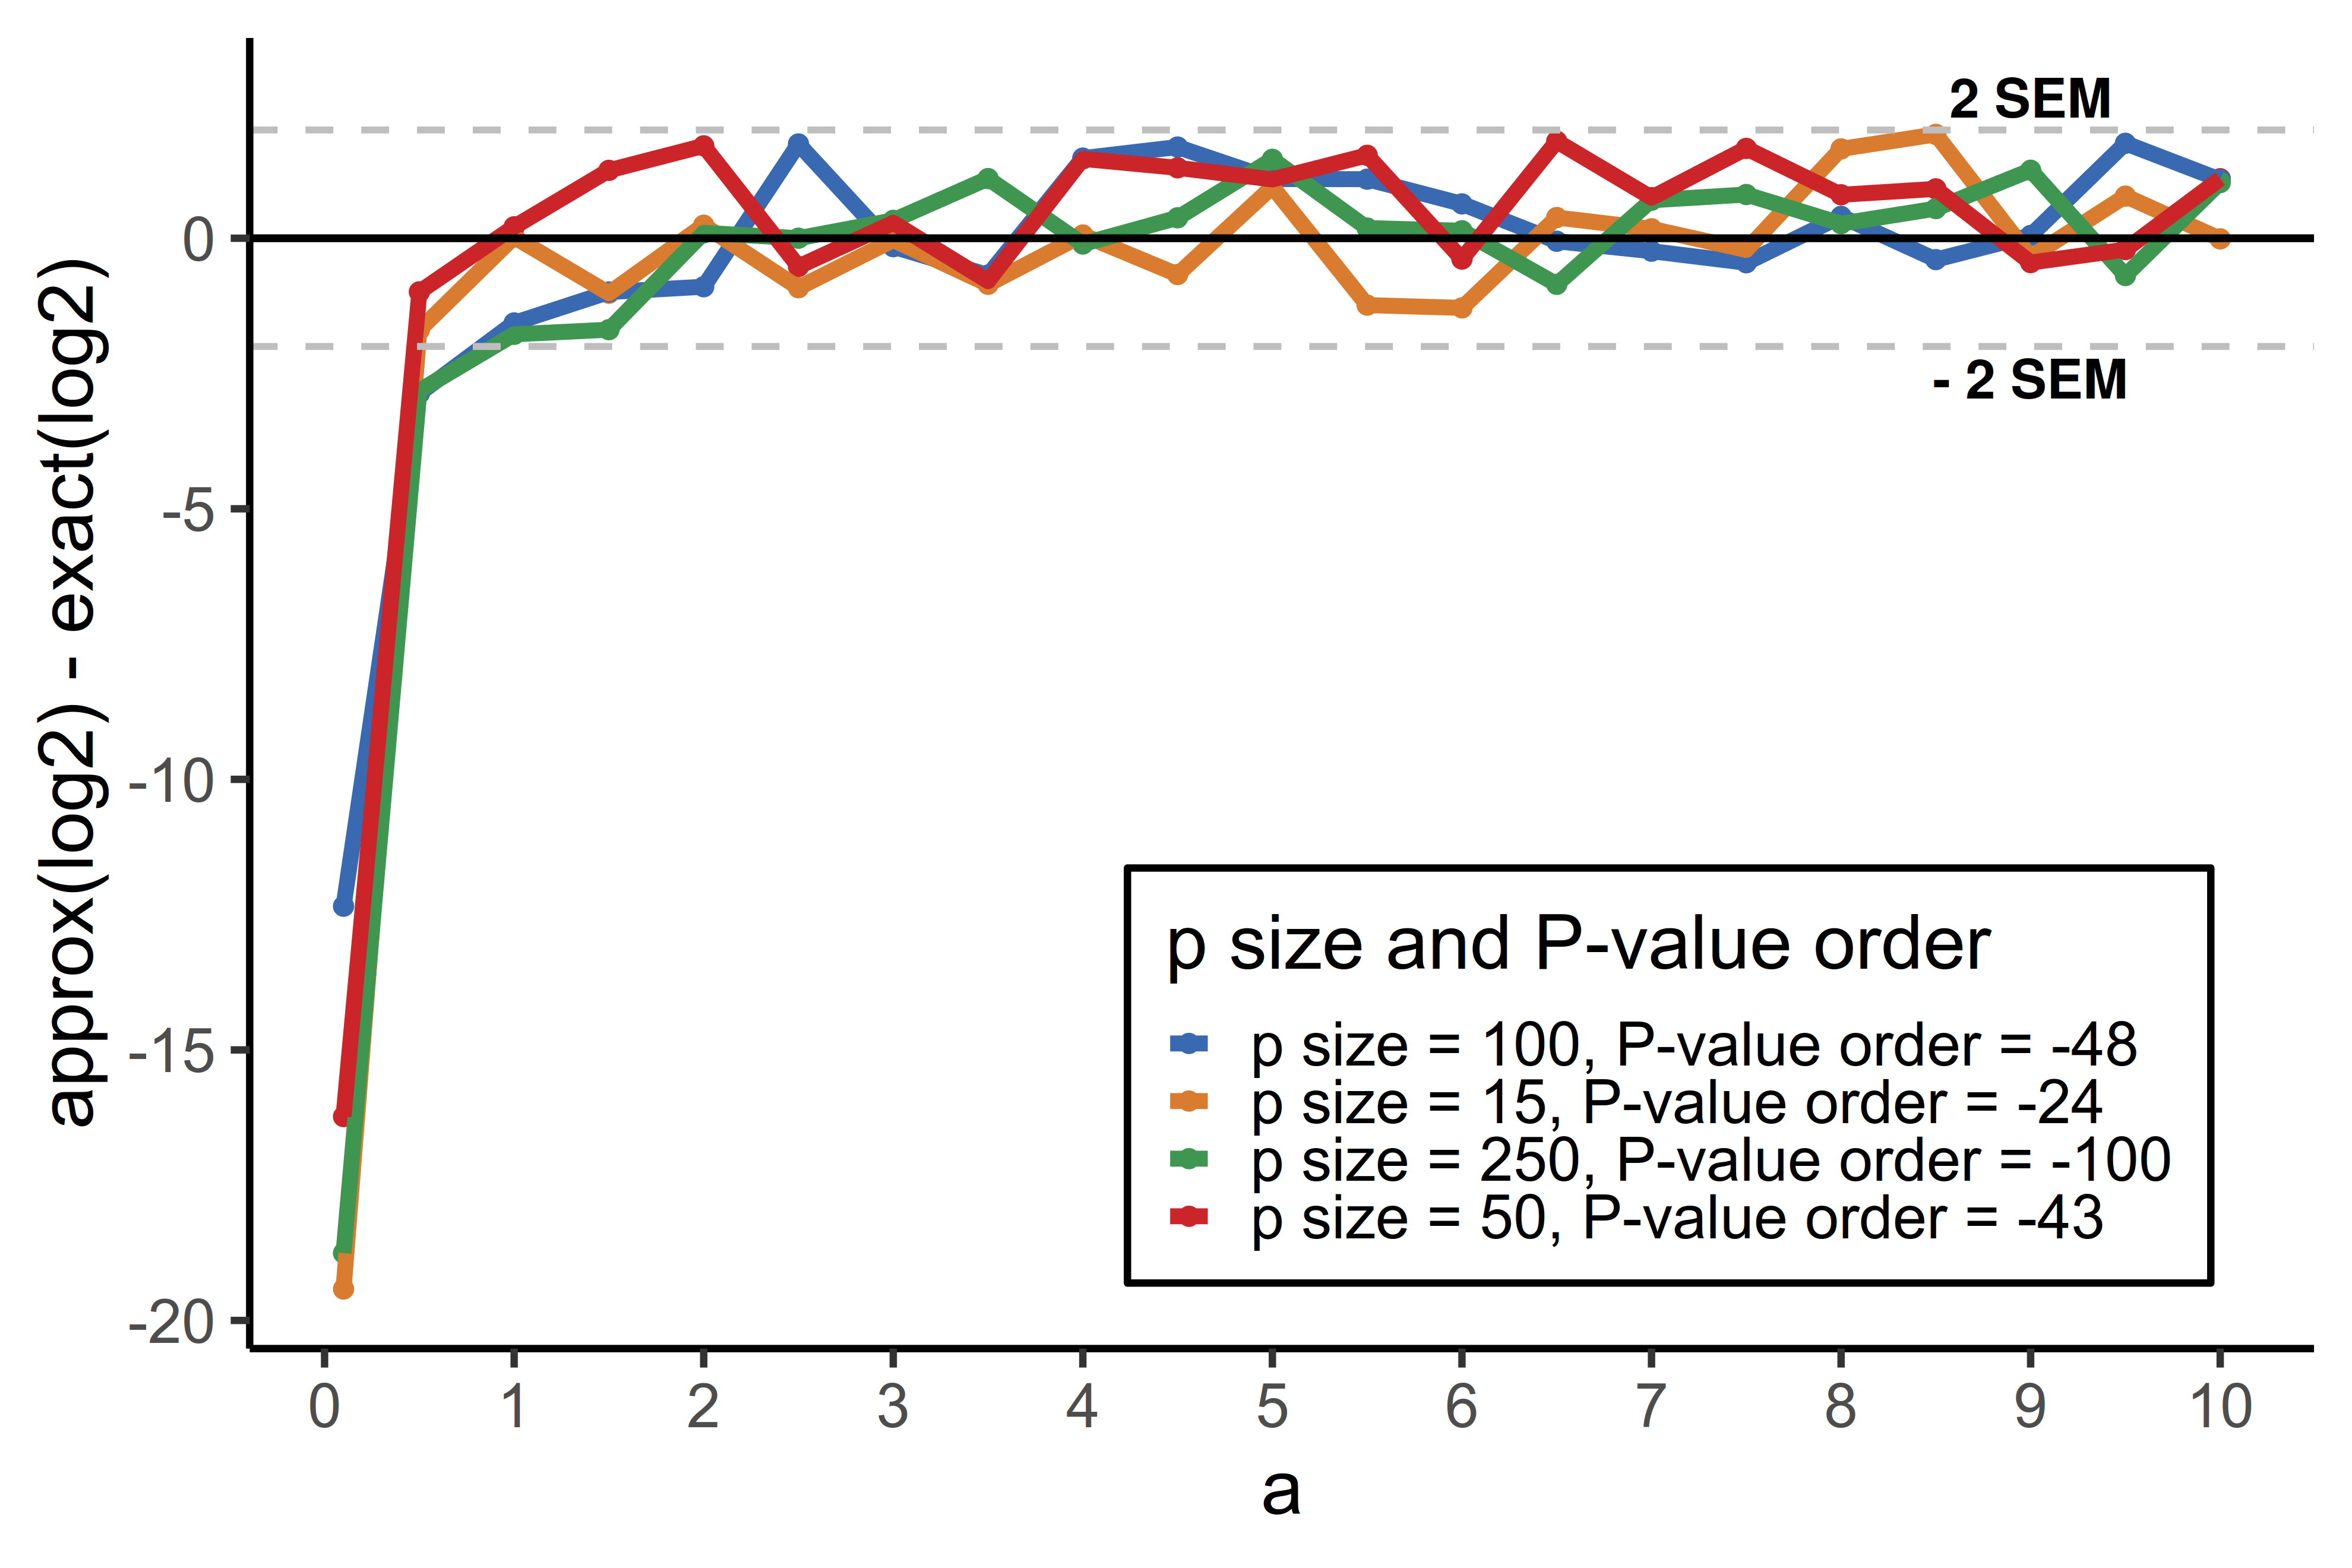
\includegraphics[width=0.65\linewidth]{multipleError_1.png}
    \centering
    \caption{Ошибка метода FGSEA-Multilevel в зависимости от числа шагов алгоритма Метрополиса}
    \label{fig:pval_error}
\end{figure}

В результате был предложен подход оценивания вероятностей редких событий при проверке статистических гипотез для наборов генов.
Подход был апробирован за счет реализации метода FGSEA-Multilevel, который решает задачу анализа представленности функциональных наборов генов.

В \textbf{третьей главе} определена оригинальная статистика, которая может быть применена для экспериментов со сложным дизайном.
Она послужила основой для метода GESECA, который позволяет проводить проверку статистических гипотез для наборов генов и числовой матрицы экспрессии без требования наличия аннотации образцов.

В случае наличия более чем двух различных биологических групп образцов, становится невозможным прямое применение классического метода \cite{subramanian2005gene}.
Поэтому, предлагается использовать следующую величину в качестве статистики представленности для набора генов $X$:
\[
       sg(X) = \mathrm{D} \left(\frac{E^T \cdot \overrightarrow{X}}{\Vert \overrightarrow{X} \Vert}\right),
\]
где $\mathrm{D}$ обозначает дисперсию, $E$ матрица экспрессии генов (строчки соответствуют генам, столбцы соответствуют образцам) и $\overrightarrow{X}$ - вектор следующего вида
\[
    \overrightarrow{X} = \begin{cases}
        1, & \text{если i-ый ген принадлежит набору X}, \\
        0, & \text{если i-ый ген не принадлежит набору X}.
    \end{cases}
\]

После введения статистики представленности $sg(\cdot)$ можно аналогичным образом как это было осуществлено в главе 2  применить подход для оценивания редких событий для наборов генов при проверки статистических гипотез для наборов генов.
Пусть $p$ - тестируемый набор генов, тогда необходимо вычислить следующее P-значение:
\[
    \mathrm{P} \left( sg(X) \geqslant sg(p) \right). 
\] 

На практике, так же как это было и для P-значений в главе 2, не имеется аналитического выражения, которое бы сразу позволило вычислить эту вероятность.
Поэтому вводится оценка для искомой вероятности, которая вычисляется при помощи генерации выборок случайных наборов генов.
Для решения проблемы вычисления вероятностей редких событий, которые имеют экстремально малые P-значения, также применяется многоуровневый подход Монте-Карло.

В действительности, метод GESECA может быть без ограничений применен для случая экспериментов с простым дизайном.
Для таких случаев результаты работы метода GESECA находятся в хорошем соответствии с методом анализа представленности FGSEA-Multilevel (рис. \ref{fig:geseca_vs_fgsea}), который основан на использовании результатов дифференциальной экспрессии генов.

\begin{figure}[h!]
    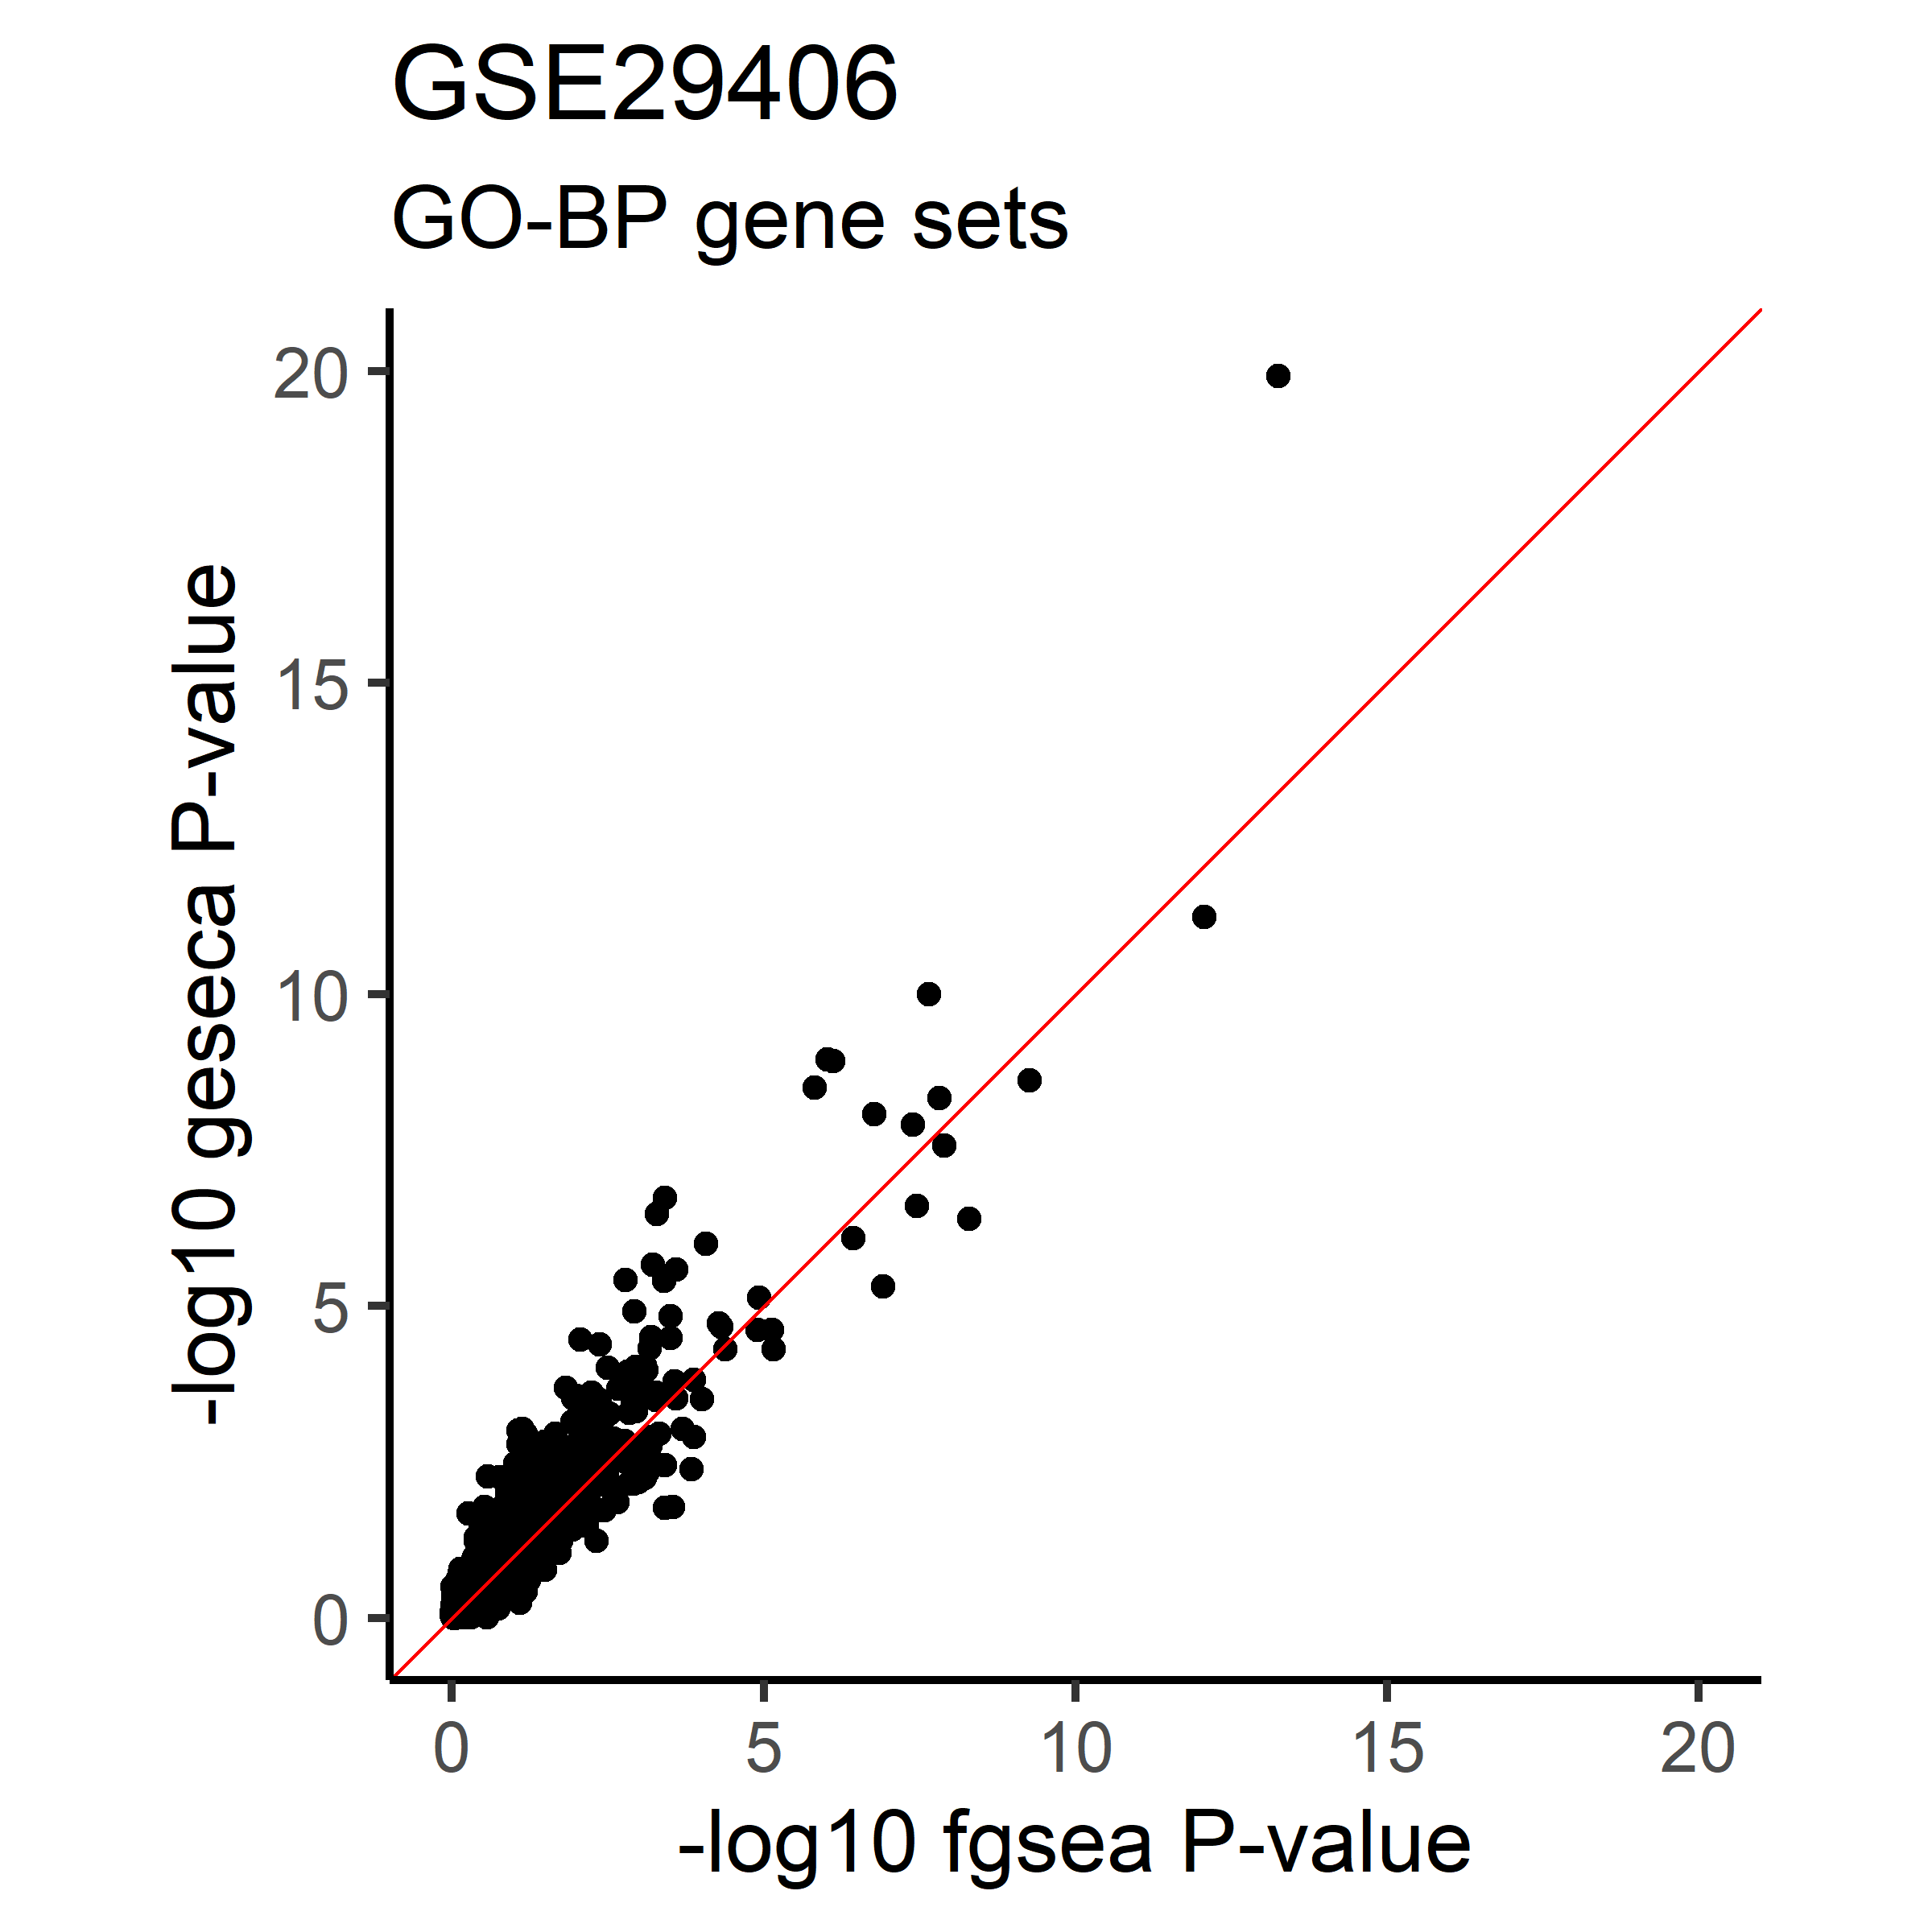
\includegraphics[width=0.4\linewidth]{GSE29406_GOBP_FGSEA_VS_GESECA.png}
    \centering
    \caption{Пример сравнения методов GESECA и FGSEA-Multilevel для эксперимента GSE29406 и коллекции наборов генов Gene Ontology Biological Process}
    \label{fig:geseca_vs_fgsea}
\end{figure}



В результате была определена статистика для наборов генов, которая позволила в автоматическом режиме проверять статистические гипотезы при анализе биологических экспериментов без требования наличия аннотации образцов.


% Можно сослаться на свои работы в автореферате. Для этого в файле
% \verb!Synopsis/setup.tex! необходимо присвоить положительное значение
% счётчику \verb!\setcounter{usefootcite}{1}!. В таком случае ссылки на
% работы других авторов будут подстрочными.
% Изложенные в третьей главе результаты опубликованы в~\cite{vakbib1, vakbib2}.
% Использование подстрочных ссылок внутри таблиц может вызывать проблемы.


В \textbf{четвертой главе} приведено описание системы поиска биологических экспериментов.
Данная система позволяет по переданному на вход набору генов найти релевантные биологические эксперименты.
Предложены подходы для оценки качества возвращаемых ранжирований экспериментов.

В качестве базы данных, внутри которой будет осуществляться поиск, было взято объединение подмножества свободно доступных экспериментов репозитория Gene Expression Omnibus (GEO, \url{https://www.ncbi.nlm.nih.gov/geo/}) и экспериментов РНК-секвенирования ARCHS4 \cite{lachmann2018massive}.
В результате база насчитывает более 50 тысяч различных экспериментов.
Доступными для поиска являются эксперименты, проведенные на людях и мышах.
При этом в среднем на каждый организм приходится по 25 тысяч экспериментов.

Входными данными для метода является набор генов, для которого требуется найти релевантные эксперименты из базы.
В качестве меры релевантности эксперимента предлагается использовать P-значение, возвращаемое методом GESECA для конкретного эксперимента и заданного набора генов.
Таким образом, для каждого эксперимента из базы данных вычисляется P-значение, которое характеризует степень совместной регуляции набора в рамках эксперимента.
Затем по полученным P-значениям производится сортировка экспериментов от меньших P-значений к большим.

Разработанная система поиска позволяет систематически переиспользовать и проводить повторный анализ для опубликованных матриц экспрессии результатов биологических экспериментов.
Для подтверждения аккуратности метода мы произвели исследование результатов работы метода на примере экспериментов CRowd Extracted Expression of Different Signatures (CREEDS) \cite{wang2016extraction}.
Для каждого эксперимента из этой коллекции в ручном режиме были сопоставлены наборы генов с высокой совместной регуляцией.
В этом анализе мы рассмотрели все упоминаемые в CREEDS эксперименты и соответствующие им наборы генов, что составило 1772 эксперимента и 3544 набора генов для экспериментов на людях и 1894 эксперимента и 3788 набора генов для экспериментов на мышах.
После этого для каждого организма и набора генов были вычислены P-значения среди всех экспериментов.
В результате истинный набор генов оказывался среди 100 самых статистически значимых в 75\% случаев.

Предложена поисковая система, которая предоставляет прямолинейный подход по систематическому переиспользованию и повторному анализу публично доступных матриц экспрессии биологических экспериментов.
Такой подход способен помочь находить новые биологические закономерности, а также подтверждать различные биологические гипотезы относительно процессов протекающих в клетках живых организмов.


\FloatBarrier
\pdfbookmark{Заключение}{conclusion}                                  % Закладка pdf
В \textbf{заключении} приведены основные результаты работы, которые заключаются в следующем:
%% Согласно ГОСТ Р 7.0.11-2011:
%% 5.3.3 В заключении диссертации излагают итоги выполненного исследования, рекомендации, перспективы дальнейшей разработки темы.
%% 9.2.3 В заключении автореферата диссертации излагают итоги данного исследования, рекомендации и перспективы дальнейшей разработки темы.
\begin{enumerate}
  \item В ходе работы был усовершенствован метод FGSEA-Multilevel для анализа представленности функциональных наборов ггенов. Метод основан на применении многоуровневого метода Монте-Карло и позволяет вычислять произвольно малые P-значения.
  \item Был разработан новый метод GESECA, позволяющий в автоматическом режиме проводить анализ представленности для транскриптомных данных как сложного так и простого дизайна.
  \item Реализована система для осуществления поиска релевантных биологических экспериментов по заданному набору генов.
\end{enumerate}


\pdfbookmark{Литература}{bibliography}                                % Закладка pdf
% При использовании пакета \verb!biblatex! список публикаций автора по теме
% диссертации формируется в разделе <<\publications>>\ файла
% \verb!common/characteristic.tex!  при помощи команды \verb!\nocite!

\ifdefmacro{\microtypesetup}{\microtypesetup{protrusion=false}}{} % не рекомендуется применять пакет микротипографики к автоматически генерируемому списку литературы
\urlstyle{rm}                               % ссылки URL обычным шрифтом
\ifnumequal{\value{bibliosel}}{0}{% Встроенная реализация с загрузкой файла через движок bibtex8
    \renewcommand{\bibname}{\large \bibtitleauthor}
    \nocite{*}
    \insertbiblioauthor           % Подключаем Bib-базы
    %\insertbiblioexternal   % !!! bibtex не умеет работать с несколькими библиографиями !!!
}{% Реализация пакетом biblatex через движок biber
    % Цитирования.
    %  * Порядок перечисления определяет порядок в библиографии (только внутри подраздела, если `\insertbiblioauthorgrouped`).
    %  * Если не соблюдать порядок "как для \printbibliography", нумерация в `\insertbiblioauthor` будет кривой.
    %  * Если цитировать каждый источник отдельной командой --- найти некоторые ошибки будет проще.
    \nocite{ica2020}
    \nocite{alexeev2020markov}
    \nocite{kmu_rints_2019}
    \nocite{spisok_2019}
    \nocite{kmu_2019}
    \nocite{mccmb_2019}
    \nocite{cshl_2020}
    \nocite{mccmb_2021_fgsea}
    \nocite{mccmb_2021_geseca}

    \ifnumgreater{\value{usefootcite}}{0}{
        \begin{refcontext}[labelprefix={}]
            \ifnum \value{bibgrouped}>0
                \insertbiblioauthorgrouped    % Вывод всех работ автора, сгруппированных по источникам
            \else
                \insertbiblioauthor      % Вывод всех работ автора
            \fi
        \end{refcontext}
    }{
        \ifnum \totvalue{citeexternal}>0
            \begin{refcontext}[labelprefix=A]
                \ifnum \value{bibgrouped}>0
                    \insertbiblioauthorgrouped    % Вывод всех работ автора, сгруппированных по источникам
                \else
                    \insertbiblioauthor      % Вывод всех работ автора
                \fi
            \end{refcontext}
        \else
            \ifnum \value{bibgrouped}>0
                \insertbiblioauthorgrouped    % Вывод всех работ автора, сгруппированных по источникам
            \else
                \insertbiblioauthor      % Вывод всех работ автора
            \fi
        \fi
        %  \insertbiblioauthorimportant  % Вывод наиболее значимых работ автора (определяется в файле characteristic во второй section)
        \begin{refcontext}[labelprefix={}]
            \insertbiblioexternal            % Вывод списка литературы, на которую ссылались в тексте автореферата
        \end{refcontext}
        % Невидимый библиографический список для подсчёта количества внешних публикаций
        % Используется, чтобы убрать приставку "А" у работ автора, если в автореферате нет
        % цитирований внешних источников.
        \printbibliography[heading=nobibheading, section=0, env=countexternal, keyword=biblioexternal, resetnumbers=true]%
    }
}
\ifdefmacro{\microtypesetup}{\microtypesetup{protrusion=true}}{}
\urlstyle{tt}                               % возвращаем установки шрифта ссылок URL
